%Template Poster in LaTeX
%Departemen Teknik Elektro dan Informatika
%Sekolah Vokasi UGM

%Dikembangkan oleh Dr. Ir. Fahmizal, S.T., M.Sc. dan Tim

%Perangkat lunak yang digunakan untuk mengolah LaTeX pada template ini adalah
%- TeXstudio
%- MiKTex
%- Overleaf (LaTEX editor berbasis daring)


\documentclass{PosterRisetFMZ}

% optional, makes QR code clickable
\usepackage[hidelinks,implicit=false,bookmarks=false]{hyperref}

\usepackage{amsmath}

\title{Dr. Ir. Fahmizal Research's Groups}

\addauthornote{mail}[]{\ttfamily Instrumentation and Control Engineering Technology}


\addauthor[mail]{Lecturer and Researcher in Vocational College Universitas Gadjah Mada}

\addfootimage(c:right column.center)[http://fahmizal.staff.ugm.ac.id]{Logo UGM}

\addfootimage(c:left  column.center)[http://otomasi.sv.ugm.ac.id]{menara ilmu otomasi}

\newlength{\textboxwidth}
\newlength{\textboxcolumnsep}\setlength{\textboxcolumnsep}{1em}

\setlength\arrayrulewidth{2pt}
\def\centeredhrulefill{\leaders\hbox{\rule[.5ex]{5pt}{\arrayrulewidth}}\hfill}

% source: http://tex.stackexchange.com/questions/23100/looking-for-an-ignorespacesandpars
\makeatletter
\def\ignorespacesandpars{%
  \begingroup
  \catcode13=10
  \@ifnextchar\par
    {\endgroup\expandafter\ignorespacesandpars\@gobble}%
    {\endgroup}%
}
\makeatother

\def\textbox(#1) at (#2) [#3] <#4,#5> title #6{%
  \def\textboxname{#1}%
  \def\textboxpos{#2}%
  \def\textboxalign{#3}%
  \def\textboxncolumns{#4}%
  \setlength{\textboxwidth}{#5}%
  \def\textboxtitle{#6}%
%
  \ifdefstring{\textboxncolumns}{1}{%
    % single column
    \def\atbeginofminipage{%
      \vspace{.5\baselineskip}%
      \par\noindent\ignorespacesandpars}%
    \def\atendofminipage{}%
  }{%
    % multiple columns
    \setlength{\textboxwidth}{\textboxncolumns\textboxwidth}%
    \addtolength{\textboxwidth}{\textboxncolumns\textboxcolumnsep}%
    \addtolength{\textboxwidth}{-\textboxcolumnsep}%
    \def\atbeginofminipage{%
      \setlength{\columnsep}{1em}%
      \begin{multicols}{\textboxncolumns}%
        \par\noindent\ignorespacesandpars}%
    \def\atendofminipage{%
      \end{multicols}}%
  }%
%
  \node[inner sep=0pt,outer sep=0cm] (#1) at (#2) [#3] \bgroup%
    \begin{minipage}{\textboxwidth}%
      \setlength{\parskip}{0pt}%
      \setlength{\parindent}{1em}%
      \par\noindent%
      {% title
        \color{tudcyan}\rm\scshape%
        \centeredhrulefill\hspace{1em}%
        \textboxtitle%
        \hspace{1em}\centeredhrulefill}%
      \atbeginofminipage}%
\def\endtextbox{%
      \atendofminipage%
    \end{minipage}%
  \egroup;%
}

\begin{document}
\begin{tikzpicture}[remember picture,overlay,line width=\arrayrulewidth]

\begin{textbox}(introduction)
at (body.north west) [below right] <1,24cm>
title {Pendahuluan}

Tawaran diberikan kepada mahasiswa Teknologi Rekayasa Instrumentasi dan Kontrol angkatan 2021 untuk dapat melakukan riset Proyek Akhir dengan Tema; Kendali dan Robotika.

\end{textbox}

\begin{textbox}(Tema Riset)
at (body.north east) [below left] <2,24cm>
title {Tema Riset}

  \begin{itemize}
    \item Robot Operating System (ROS) 
    \item Arm Robots
    \item Humanoid Robots
    \item Unmanned Aerial Vehicle (UAV)
    \item Optimal Control
    \item Adaptive Control
    \item Reinforcement Learning Control
    \item Rocket Control Simulation
    
  \end{itemize}

\end{textbox}

\begin{textbox}(Alumni)
at ([shift={(0pt,-12cm)}]body.north west) [below right] <1,77cm>
title {Kualifikasi Mahasiswa}

  \begin{itemize}
	\item Memiliki pemahaman dasar elekronika dan kendali yang baik.
	\item Terampil menggambar desain elektronika dan mencetak PCB.
	\item Terampil menggambar desain mekanika.
	\item Memiliki dasar kemampuan pemrograman Arduino, Python, ROS, MATLAB, dan LaTeX.
	\item Kuat mental, tidak mudah mengeluh, pekerja keras.
	\item Mau melakukan penelitian di lingkungan Lab, berkegiatan \textit{hands on skill} seperti soldering, 3D printing, dan laser cutting.
\end{itemize}
\begin{center}
	\begin{figure}
	\centering
	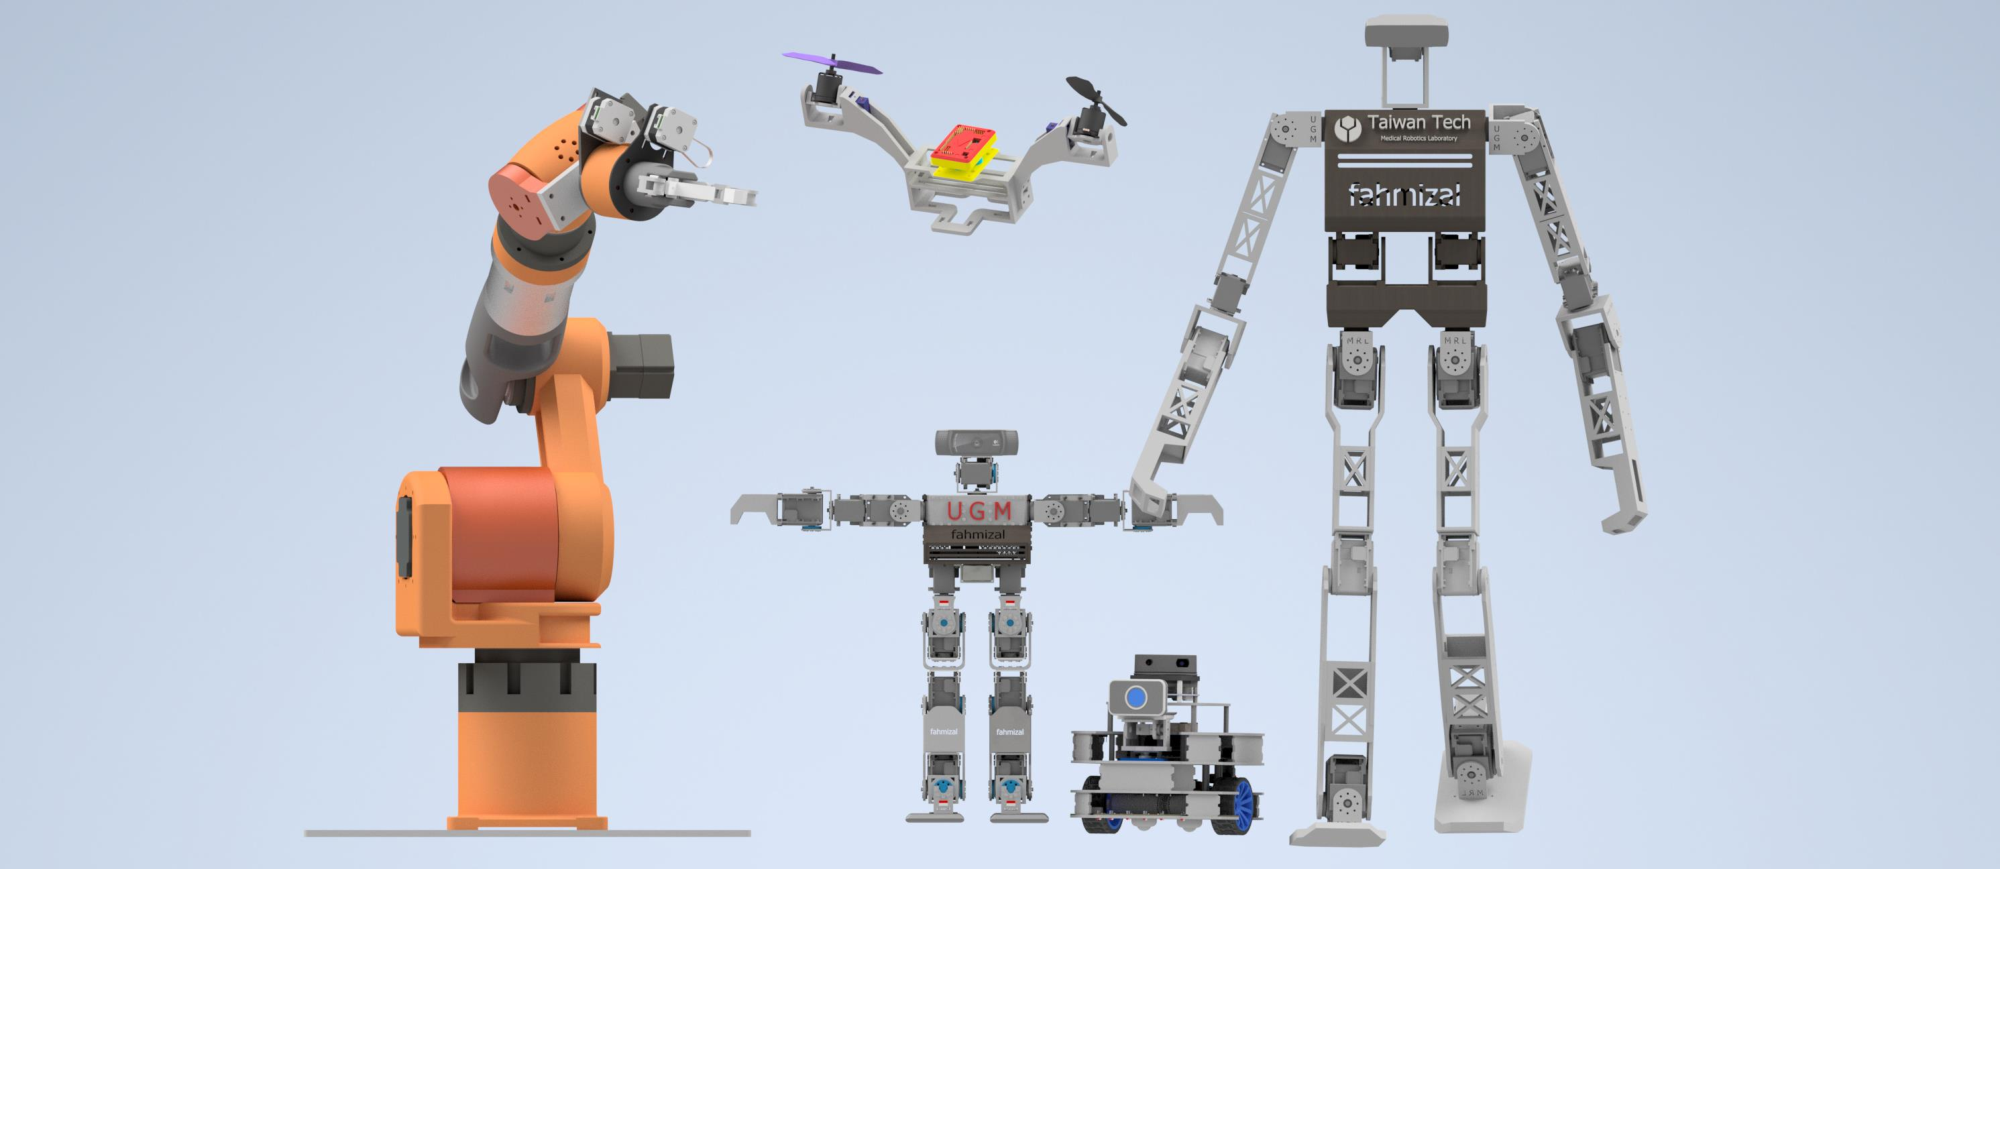
\includegraphics[width=0.95\linewidth]{Dr Fahmizal Riset.pdf}
	\end{figure}
\end{center}

\end{textbox}

\begin{textbox}(Benefits)
at (body.south west) [above right] <1,35cm>
title {Benefits}%

  \begin{itemize}
	\item Akan dipandu secara \textit{intensive and continue} oleh pembimbing.
	\item Diarahkan bagaimana cara menulis hasil penelitan pada Jurnal International.
	\item Fasilitas penelitian yang akan di-\textit{support} oleh pembimbing.
	\item Dilibatkan dalam kegiatan penelitian pembimbing.
	\item Berpotensi untuk lulus tepat waktu Wisuda Agustus 2025$^*$ (Waktu pengerjaan: Januari 2025 – Juli 2025)
\end{itemize}


\end{textbox}

\begin{textbox}(Alumni)
at (body.south east) [above left] <1,35cm>
title {Alumni}%

  \begin{itemize}
	\item Ahmad Jaelani Sidik (20/457190/SV/17637), Wisuda Agustus 2024 dengan IPK: 3,92; Penelitiannya terkait kendali attitude pada UAV Tricopter.
	\item Priyova Muhammad Rafief (20/457197/SV/17644), Wisuda Agustus 2024 dengan IPK: 3,87; Penelitiannya terkait ROS pada RGBD SLAM pada mobile robot.
	\item Bodhi Setiawan (20/464239/SV/18558), Wisuda November 2024 dengan IPK: 3,75; Penelitiannya terkait kendali kestabilan inverted pendulum pada mobile robot.
\end{itemize}

\end{textbox}


\end{tikzpicture}
\end{document}

